%% ****** Start of file apstemplate.tex ****** %
\documentclass[aps,prl,reprint,groupedaddress]{revtex4-2}

% You should use BibTeX and apsrev.bst for references
% Choosing a journal automatically selects the correct APS
% BibTeX style file (bst file), so only uncomment the line
% below if necessary.
% \bibliographystyle{apsrev4-2}

\usepackage{graphicx}
\usepackage{epstopdf}
\usepackage{amsmath}
\usepackage{amsthm}
\usepackage{amsfonts}
\usepackage{subfigure}
\usepackage{hhline}
\usepackage[left=1cm,right=1cm,top=1cm,bottom=1cm]{geometry}
\usepackage[miktex]{gnuplottex}
\usepackage{xcolor}
\usepackage{amssymb}
\usepackage{amsmath}
\usepackage{color}
\usepackage{hyperref}
\usepackage[percent]{overpic}
\usepackage{tikz}
\usepackage{mathrsfs}
\usepackage{wasysym}
\usepackage{tikz-cd}
\usepackage{caption}  % Elimina hypcap=true si está presente
\usepackage{stackengine,scalerel}

\usepackage{caption}
\captionsetup{skip=0pt}  % Reduce el espacio entre la imagen y su caption
\raggedbottom

% so sections, subsections, etc. become numerated.
\setcounter{secnumdepth}{3}

\newenvironment{Figura}
  {\par\medskip\noindent\minipage{\linewidth}}
  {\endminipage\par\medskip}

\renewcommand{\appendixname}{Apéndice} % Change "Appendix" to "Apéndice"

\begin{document}

%Title of paper
\title{
Análisis Numérico del modelo de Hodgkin-Huxley
}

% autores
\author{Mauricio Morán}
\email[]{maurijmoran@gmail.com}
\affiliation{}

\author{Kevin Gaston Mansilla}
\email[]{kevin.mansilla@mi.unc.edu.ar}

\author{Bruno Principi}
\email[]{principi.bruno@gmail.com}
\affiliation{}

%fecha
\date{\today}

\begin{abstract}
En este trabajo se estudia el comportamiento del voltaje de una membrana celular
simulada mediante el modelo de Hodgkin-Huxley bajo varias situaciones, como 
lo son un estumulo débil y furete, una ráfaga, un período reflectario y 
exitaciones espontaneas en respuesta al ruido. El sistema de ecuaciones del 
modelo fue resuelto mediante el método de Runge-Kutta de orden cuatro, excepto 
en el último caso que mencionamos, en el cual se utilizó el método de Euler ya 
que cuando se integran procesos estocasticos las tecnicas cambian. Los 
resultados obtenidos concuerdan con lo esperado teóricamente y se 
discuten en la sección de resultados.
\end{abstract}

% insert suggested keywords - APS authors don't need to do this
%\keywords{}

%\maketitle must follow title, authors, abstract, and keywords
\maketitle

\section{Introducción}

El modelo de Hodgkin-Huxley busca describir el potencial sobre una membrana 
celular previo, durante y después de un potencial de acción. Para ello se encarga 
de caracterizar, el voltaje $V_{m}$ de la membrana en función del tiempo $t$ y 
de parámetros como el número y tipo de bombas de sodio-potasion que permiten 
el paso de iones positivos (Na$^{+}$ y K$^{+}$) desde o hacia la parte interna 
de la célula. Lo cual genera un despolarizacion que desemboca, si se supera 
un cierto umbral en $v_{m}$, en la creación de un potencial de acción el cual 
se muestra a continuación

\begin{Figura}
    \centering
    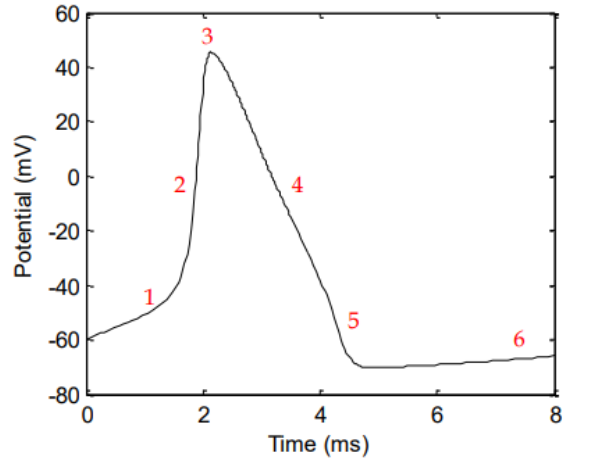
\includegraphics[width=0.7\textwidth]{figs/potencial_accion.png}
    \captionof{figure}{Voltaje $V_{m}$ vs $t$ para un potencial de acción}
    \label{fig-potencial}
\end{Figura}

En general, el potencial de equilibrio en una neurona se encuentra alrededor de 
los $-65 mV$ y se mantiene por el flujo de Na$^{+}$ hacia el exterior y de K$^{+}$ 
hacia el interior. Sim embargo, durante la aplicación de un estimulo o corriente 
externa, $V_{m}$ puede variar y despues de llegar a un valor umbral que se 
corresponde con el número $1$ de la figura \ref{fig-potencial}, se abren 
completamente los canales en la membrana que permiten el flujo de Na$^{+}$ hacia
el interior superando el flujo entrante de K$^{+}$, causando un aumento o 
despolarización en $V_{m}$ que se muestra en el número $2$ de la figura. 

Mientras el potencial aumenta se abren completamente los caneles que permiten 
la salida de K$^{+}$ fuera de la membrana, es por esto que cuanod el potencial
alcanza su máximo (punto 3), los canales que permiten la entrada de Na$^{+}$
se cierran y el potencial comienza a retornar a su valor de equilibrio (punto $4$).

Luego en $5$, los calanes que permiten la salida de los iones se cierran en un 
voltaje menor a $-65 mV$ y en $6$ se retorna al voltaje de equilibrio, cuando 
los canales de Na$^{+}$ y K$^{+}$ retornan a su estado de reposo. 
(\cite{lamberti2007desarrollo})

\section{Modelo Matemático}

En el modelo la descripción del potencial en la membrana $V_{m}$ con su 
respectiva capacitancia por unidad de área $C_{m}$ y donde se aplicaba un estimulo 
externo o corriente $I(x,t)$, due descripta un circuito eléctrico que se muestra
en la figura \ref{fig-circuito}, donde las corrientes iónicas y corrientes de 
fuga netas, se caracterizaban por capacitancias $g_{j}$ t capacitores $E_{j}$
acoplados a la membrana

\begin{Figura}
    \centering
    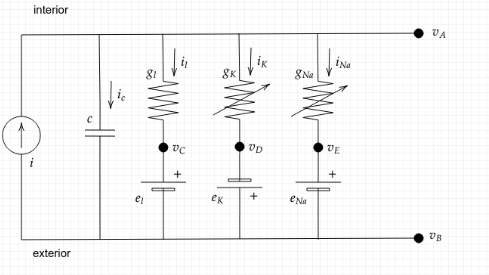
\includegraphics[width=0.8\textwidth]{figs/circuito.png}
    \captionof{figure}{Circuito que describe el potencial en la membrana}
    \label{fig-circuito}
\end{Figura}

La siguiente ecuación describe la evolución temporal del potencial de membrana
\begin{align*}
    C_m \frac{dV}{dt} = &\underbrace{I(x,t)}_{\text{corriente externa}} - \underbrace{g_{Na}(v_{m} - e_{Na})}_{\text{Corriente $Na^{+}$}}  \\
    &- \underbrace{g_{K}(v_{m} - e_{K})}_{\text{Corriente $K^{+}$}} - \underbrace{g_{L}(v_{m} - e_{L})}_{\text{corriente de fuga}}
\end{align*}

donde $C_{m}$ es la capacitancia de la membrana, $\frac{dV}{dt}$ es el potencial 
de membrana en el tiempo $t$, $I(x,t)$ es la corriente externa. $v_{m}$ es el
potencial de membrana en reposo. Las conductancias de los caneles de sodio, 
potasio y de fuga están representadas por $g_{Na}$, $g_{K}$ y $g_{L}$ mientras 
que los potenciales de equilibrio para estos mismos iones son $e_{Na}$, $e_{K}$ 
y $e_{L}$.

Ademas Hodgkin y Huxley postularon que las conductancion del sodio y del potasio 
dependían del tiempo y del potencial de membrana. Por lo que introdujeron variables 
adimensionales $m$, $n$ y $h$ que describen la probabilidad de que los canales de
sodio y potasio estén abiertos o cerrados. Estas variables evolucionan de acuerdo a
las siguientes ecuaciones diferenciales
\begin{align*}
    \frac{dm}{dt} &= \alpha_{m}(V)(1 - m) - \beta_{m}(v)m \\
    \frac{dn}{dt} &= \alpha_{n}(V)(1 - n) - \beta_{n}(v)n \\
    \frac{dh}{dt} &= \alpha_{h}(V)(1 - h) - \beta_{h}(v)h
\end{align*}

donde $\alpha_{k}$ y $\beta_{k}$ con $k \in \{m, n, h\}$ son constantes de velocidad 
de cambio de canales abiertos a cerrados y de cerrados a abiertos, respectivamente. 

Entonces el modelo completo es:
\begin{align*}
    C_{m} \frac{dV_{m}}{dt} = &I(x,t) - g_{Na}m^{3}(v_{m} - e_{Na})  \\
    &- g_{K}n^{4}(v_{m} - e_{K}) - g_{L}(v_{m} - e_{L}) \\
\end{align*}

donde 
\begin{align*}
    \frac{dm}{dt} &= \alpha_{m}(V)(1 - m) - \beta_{m}(v)m \\
    \frac{dn}{dt} &= \alpha_{n}(V)(1 - n) - \beta_{n}(v)n \\
    \frac{dh}{dt} &= \alpha_{h}(V)(1 - h) - \beta_{h}(v)h
\end{align*}

con 
\begin{align*}
    \alpha_{m}(V) &= \frac{0.1(25 - V)}{\exp\left(-\frac{25-V}{10}\right)-1} \\
    \beta_{m}(V) &= 4\exp\left(-\frac{V}{18}\right) \\
    \alpha_{n}(V) &= \frac{0.01(10 - V)}{\exp\left(\frac{10-V}{10}\right)-1} \\
    \beta_{n}(V) &= 0.125\exp\left(-\frac{V}{80}\right) \\
    \alpha_{h}(V) &= 0.07\exp\left(-\frac{V}{20}\right) \\
    \beta_{h}(V) &= \frac{1}{1 + \exp\left(-\frac{30-V}{10}\right)}
\end{align*}

y los valores de los parámetros obtenidos experimentalmente son:
\begin{align*}
    C_{m} &= 1 \mu F/cm^{2} \\
    g_{Na} &= 120 mS/cm^{2} \\
    g_{K} &= 36 mS/cm^{2} \\
    g_{L} &= 0.3 mS/cm^{2} \\
    E_{Na} &= 120 mV \\
    E_{K} &= -12 mV \\
    E_{L} &= -10.6 mV \\
    i(t) &= 10 \mu A/cm^{2}\\
    t &= 5 ms
\end{align*}

Nosotros resolveremos este sistema de ecuaciones mediante el método numérico de
Runge-Kutta de cuarto orden y analizaremos los resultados obtenidos en la
siguiente sección.

\section{Resultados}

Para implementar la solución del sistema de ecuaciones diferenciales acopladas 
se uso el método de Runge-Kutta de cuarto orden para los casos de corriente 
externa con estimulo débil y fuerte, una ráfaga, un período reflectario. Y para 
el caso de exitaciones espontaneas en respuesta al ruido se utilizó el método de
Euler.

\subsection{EL estado estacionario}

El estado estacionario del modelo se caracteriza por la anulación de las 
derivadas temporales de las variables $m$, $n$ y $h$. Para ver como se comporta 
esta situación se obtuvo el comportamiento de $m$, $n$ y $h$ en función de $V$.
El resultado se muesta en la figura \ref{fig-nmh-ee}. Tal como se esperaba 
como son probabilidades de apertura de los canales en presencia de un determinado 
voltaje, los valores de cada uno se encuentran entre $0$ y $1$. Además se observa 
como la apertura de los caneles tipo $n$ y $m$ por donde transitan los iones 
potasio y sodio, aumenta con el voltaje de la membrana. Por otro lado, un 
comportamiento contrario se obtiene para la probabilidad de apertura del canal 
tipo $h$ sonde ciculan los iones de sodio.

\begin{Figura}
    \centering
    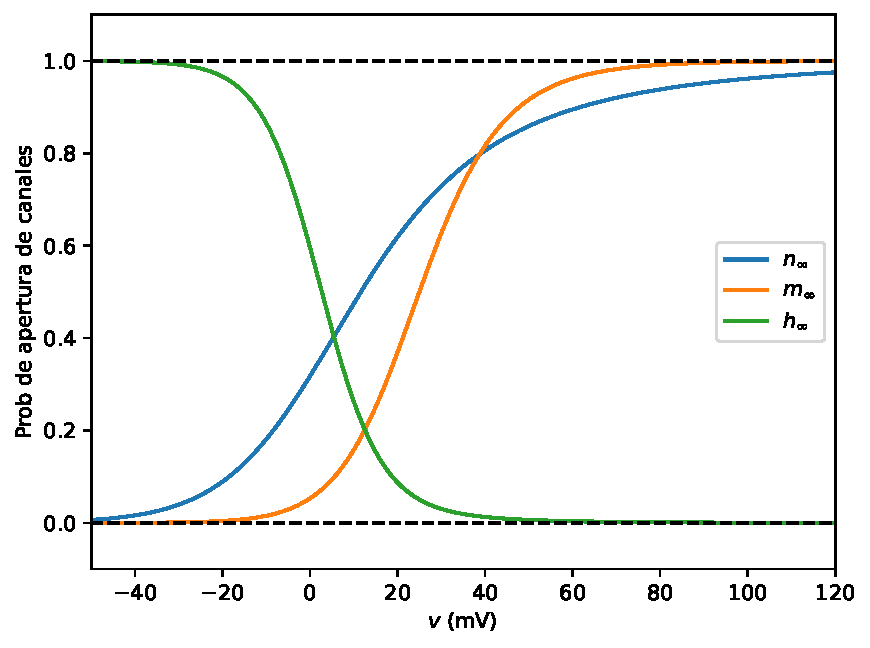
\includegraphics[width=0.8\textwidth]{figs/nmh_ee.pdf}
    \captionof{figure}{Comportamiento de $m$, $n$ y $h$ en función de $V$ para 
    estado estacionario.}
    \label{fig-nmh-ee}
\end{Figura}

La figura anteior no es muy ilustrativa para representar el potencial de acción, 
pues la definción del mismo implica un cambio en $V$ con respecto al tiempo. Es 
por ello que en las siguientes secciones se estudiarán las caracteristicas de los 
potenciales de accion en respuesta a diferentes estimulos.

\subsection{Corriente externa nula}
Al hacer la corriente externa nula, por Runge Kutta se obtiene la siguiente 
figura \ref{fig-potencial-nula}, donde se observa como el voltaje alcanza un estado de
equilibrio alrededor de los $-12 mV$. al no tener estímulos externos aparte del 
ingreso de iones de sodio y potasio, para los cuales las probabilidad de apertura 
de las puertas tambien alcanzan un valor de equilibrio como lo muestra la 
figura \ref{fig-nmh-nula}.

\begin{Figura}
    \centering
    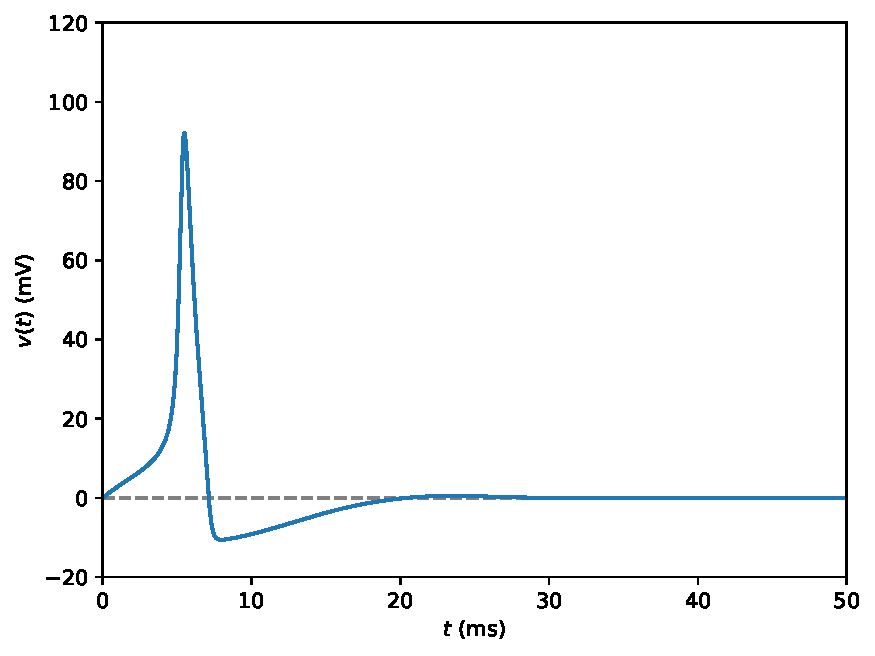
\includegraphics[width=0.7\textwidth]{figs/potencial_vs_t.pdf}
    \captionof{figure}{$V$ vs $t$ para el caso sin corriente externa, y 
    condiciones iniciales $V, n, m, h =0$ }
    \label{fig-potencial-nula}
\end{Figura}

\begin{Figura}
    \centering
    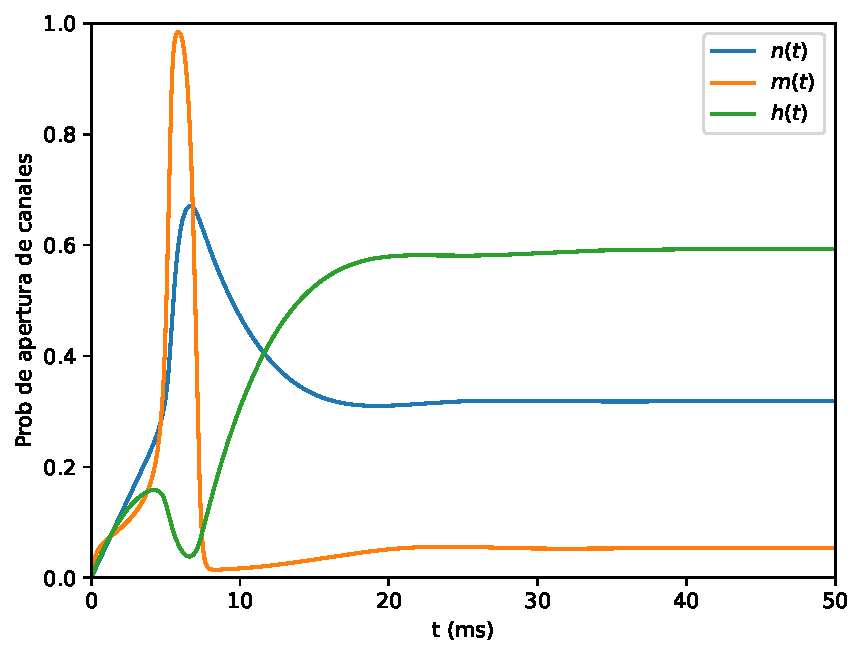
\includegraphics[width=0.7\textwidth]{figs/nmh_corriente_externa.pdf}
    \captionof{figure}{$n, m, h$ para el caso sin corriente externa, y 
    condiciones iniciales $V, n, m, h =0$ }
    \label{fig-nmh-nula}
\end{Figura}

\subsection{Estimulo débil y estimulo fuerte}

En la siguiente figura \ref{fig-potencial-df} se muestra el comportamiento del
potencial de membrana en respuesta a un estimulo débil y fuerte. En el caso del 
estimulo débil a los 2.5 ns, el potencial de membrana no alcanza el umbral 
necesario para generar un potencial de acción, mientras que en el caso del 
estimulo fuerte (10 ns), el potencial de membrana supera el umbral y se genera un 
potencial de acción.
\begin{Figura}
    \centering
    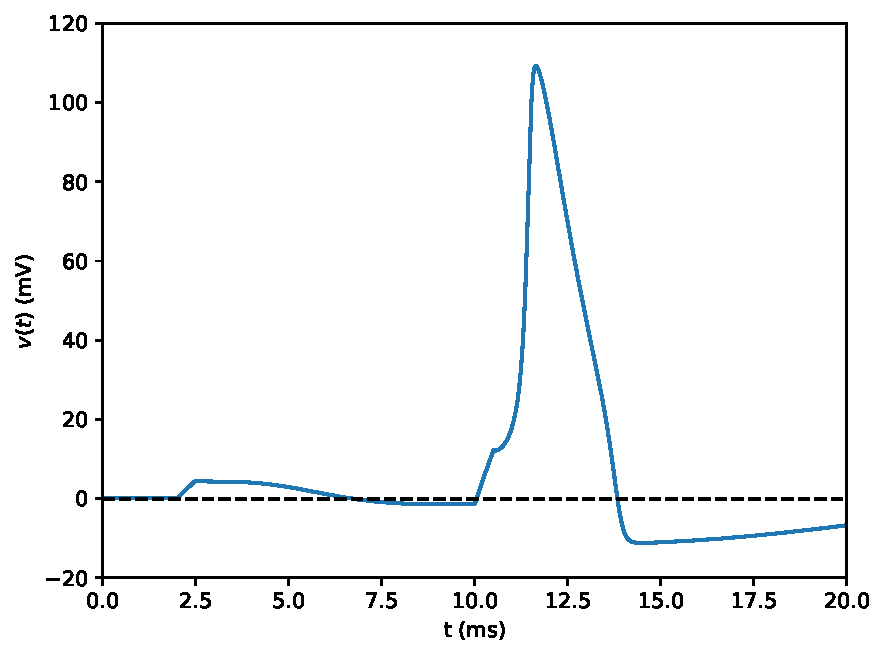
\includegraphics[width=0.7\textwidth]{figs/potencial_mem_estimulo_d_f.pdf}
    \captionof{figure}{$V$ vs $t$ de un estimulo débil y fuerte}
    \label{fig-potencial-df}
\end{Figura}

Lo mismo ocurre con las variables $n$, $m$ y $h$ que se muestran en la figura 
\ref{fig-nmh-df}. En el caso del estimulo débil, las variables apenas cambian 
debido a la corriente aplicada y luego de los 10ns cuando se aplica el estimulo
fuerte $m(t)$ sube rapidamente, activando los calanes de sodio y permitiendo la 
despolarizacion. $h(t)$ baja para desactivar los canales de sodio y $n(t)$ sube
mas lentamente para activar los canales de potasio, contribuyendo a la repolarización 
y la hiperlolarización de la membrana.
\begin{Figura}
    \centering
    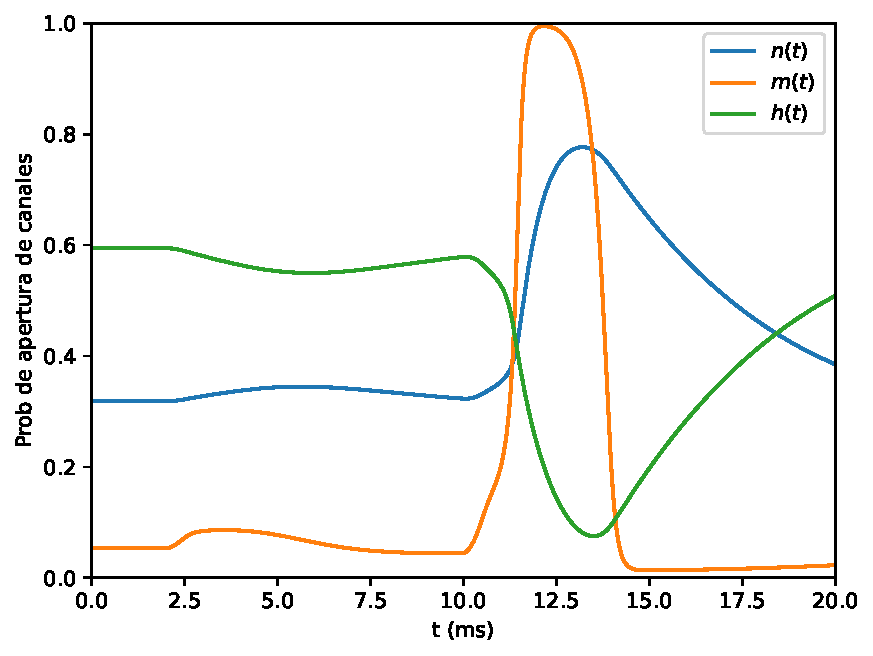
\includegraphics[width=0.7\textwidth]{figs/nmh_estimulo_d_f.pdf}
    \captionof{figure}{$n, m, h$ para el caso de un estimulo débil y fuerte}
    \label{fig-nmh-df}
\end{Figura}

\subsection{Ráfaga}

Con un estimulo tipo ráfaga, de $10 /mu A/cm^{2}$ a partir de $t=5$ como lo muestra 
la figura \ref{fig-potencial-r}, es claro que el estimulo es suficiente para
que la neurona este en estado activo durante un tiempo prolongado. Lo mismo se 
observa en la figura \ref{fig-nmh-r} donde las variables $n$, $m$ y $h$ se
mantienen en un estado activo durante un tiempo prolongado.
\begin{Figura}
    \centering
    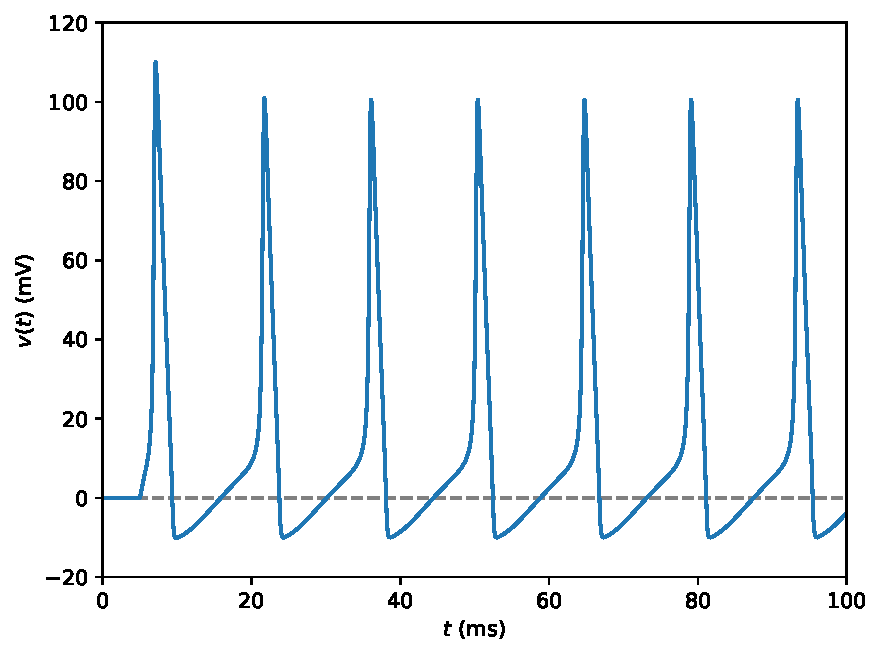
\includegraphics[width=0.7\textwidth]{figs/potencial_rafaga.pdf}
    \captionof{figure}{$V$ vs $t$ para el caso de una ráfaga}
    \label{fig-potencial-r}
\end{Figura}

\begin{Figura}
    \centering
    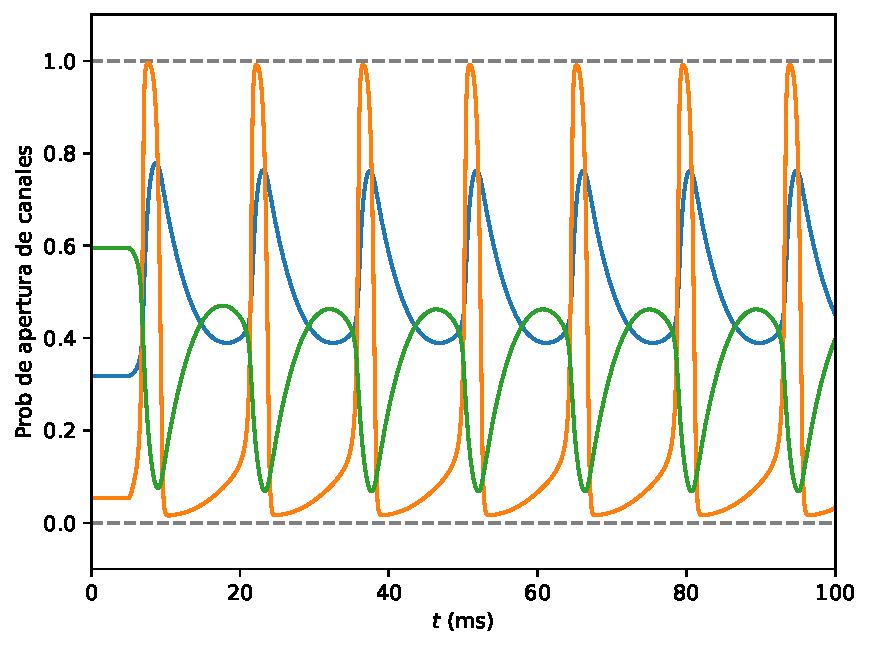
\includegraphics[width=0.7\textwidth]{figs/nmh_rafaga.pdf}
    \captionof{figure}{$n, m, h$ para el caso de una ráfaga}
    \label{fig-nmh-r}
\end{Figura}

\subsection{Período reflectario}

Por otro lado si el estimulo es un período reflectario, como se muestra en la
figura \ref{fig-potencial-reflec}, se observa que el potencial de membrana no 
alcanza el umbral necesario para generar un potencial de acción para determinados 
periodos de tiempo, pero para los $t$ que son multiplos de $10$ ns, el potencial
de membrana supera el umbral y se genera un potencial de acción. Lo mismo ocurre
con las variables $n$, $m$ y $h$ que se muestran en la figura \ref{fig-nmh-reflec}.
\begin{Figura}
    \centering
    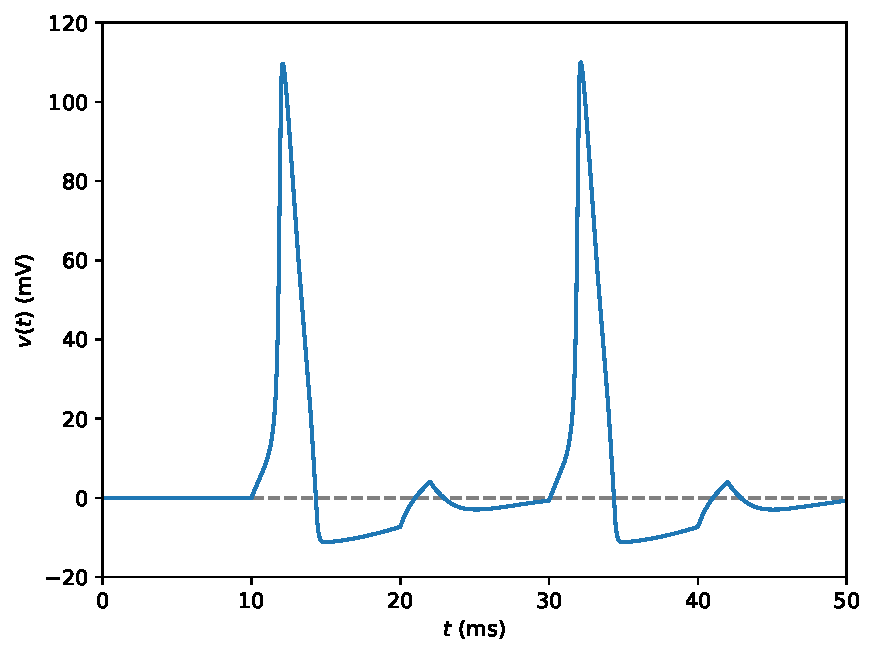
\includegraphics[width=0.7\textwidth]{figs/potencial_reflectario.pdf}
    \captionof{figure}{$V$ vs $t$ para el caso de un período reflectario}
    \label{fig-potencial-reflec}
\end{Figura}

\begin{Figura}
    \centering
    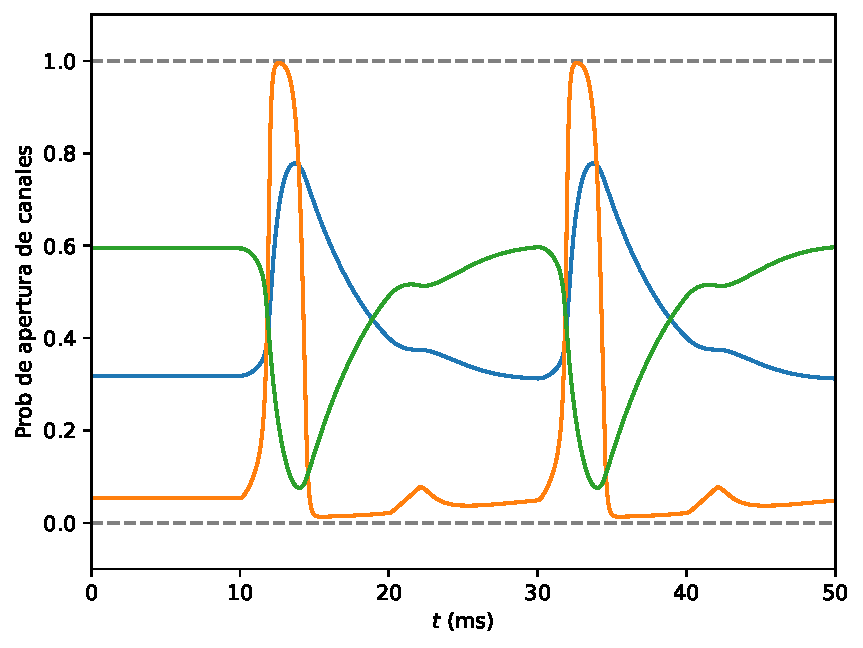
\includegraphics[width=0.7\textwidth]{figs/nmh_reflectario.pdf}
    \captionof{figure}{$n, m, h$ para el caso de un período reflectario}
    \label{fig-nmh-reflec}
\end{Figura}

\subsection{Exitaciones espontaneas en respuesta al ruido}

Por último, con exitaciones espontaneas en respuesta al ruido, es decir, una 
corriente estocástica con distribución normal estandar, el comportamiento del 
potecial de membrana se observa que hay un comportamiento oscilatorio en el
potencial de membrana, es decir, la neurona se encuentra en un estado activo
durante un tiempo prolongado, como se muestra en la figura \ref{fig-potencial-euler}.

\begin{Figura}
    \centering
    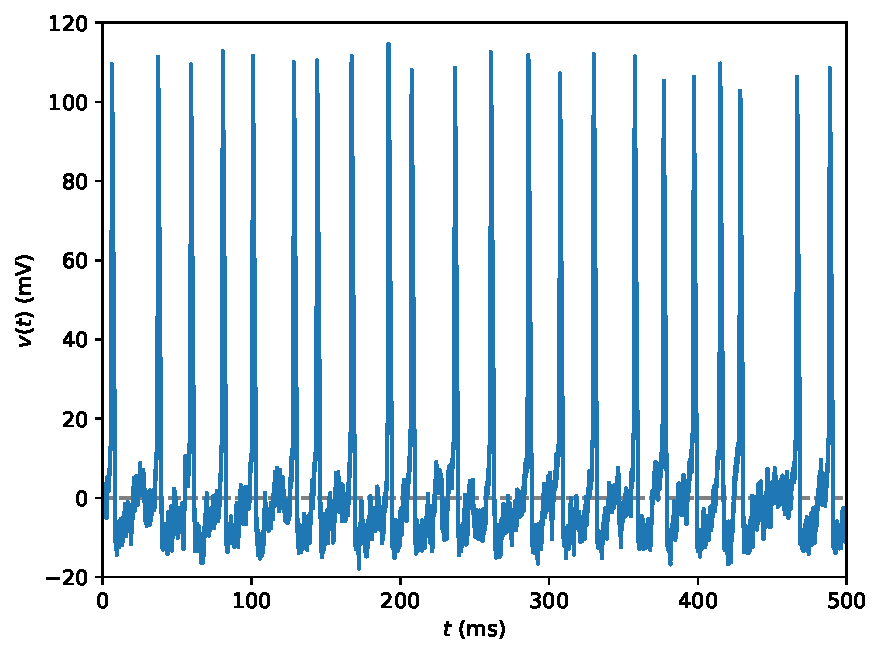
\includegraphics[width=0.7\textwidth]{figs/potencial_euler.pdf}
    \captionof{figure}{$V$ vs $t$ para el caso de exitaciones espontaneas en 
    respuesta al ruido}
    \label{fig-potencial-euler}
\end{Figura}

En cuanto a las variables $n$, $m$ y $h$ la figura \ref{fig-nmh-euler} también 
muestra un comportamiento oscilatorio.
\begin{Figura}
    \centering
    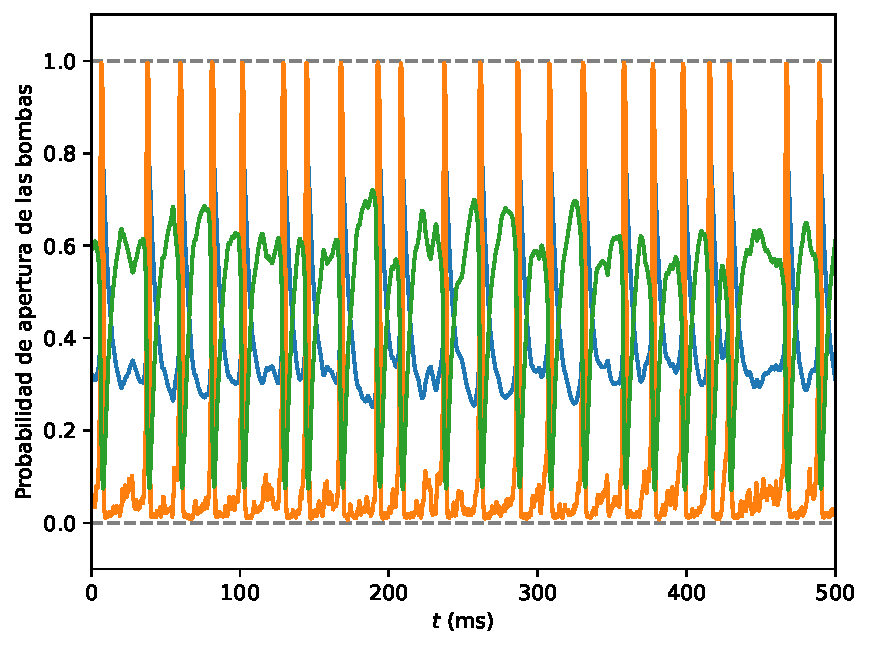
\includegraphics[width=0.7\textwidth]{figs/nmh_euler.pdf}
    \captionof{figure}{$n, m, h$ para el caso de exitaciones espontaneas en
    respuesta al ruido}
    \label{fig-nmh-euler}
\end{Figura}

\section{Conclusiones}

En este trabajo se resolvio el modelo de Hodgkin-Huxley al cual aplicamos 
diferentes estimulos para estudiar el comportamiento del potencial de membrana
en respuesta a estos. 

En ausencia de estimulos de corriente externos, se encontró como el potencial de 
membrana alcanza un estado de equilibrio alrededor de los $-12 mV$, indicando 
la existencia de un voltaje de equilibrio, para el cual las probabilidad de 
apertura de los canales por donde fluyen los iones de sodio y potasio se manienen 
constantes en el tiempo.

En presencia de estimulos débiles y fuertes, se observó como el potencial de
membrana cuando el estimulo es débil no alcanza el umbral necesario para generar
un potencial de acción, mientras que en el caso de un estimulo fuerte si lo 
alcanza. Cuando estamos en presencia de una ráfaga, el potencial de membrana se
mantiene activo durante un tiempo prolongado. En el caso de un período reflectario 
el potencial de membrana no alcanza el umbral necesario para generar un potencial
de acción para determinados periodos de tiempo, pero para los $t$ que son
multiplos de $10$ ns, el potencial de membrana supera el umbral y se genera un
potencial de acción. Por último, con exitaciones espontaneas en respuesta al ruido,
el comportamiento del potencial de membrana es oscilatorio, es decir, la neurona
se encuentra en un estado activo durante un tiempo prolongado.
% Create the reference section using BibTeX:
\bibliography{ref}

% Specify following sections are appendices. Use \appendix* if there
% only one appendix.

%\onecolumngrid


\end{document}
%
% ****** End of file apstemplate.tex ******